A hydraulic system is used to move a mass of 1 kg, but between the mass and the hydraulic system is a flexible connector, represented by the spring and damper, with $k=1$  and $b=2$. The linearized servo valve equation is $\delta q = 3 \delta x - 2 \delta p$, the piston area is $1$ m$^2$. The block diagram that represents the hydraulic system is shown below, where $N(s)=\frac{\delta Y(s)}{\delta F(s)}$ is the mechanical impedance of the load.  Find the transfer function for the load, plug it into the block diagram, and then simplify the block diagram to find the transfer function $\delta Y(s)/\delta X(s)$. 
\begin{center}
\resizebox{2.5in}{!}{
\begin{tikzpicture}[sysblock/.style={draw,rectangle,inner sep=2pt,minimum width=1cm,minimum height=1cm,very thick}]


% tank
\draw[very thick] (0,0) -- ++(2,0) -- ++(0,-.5) -- ++(1,.5) -- ++(2,0) -- ++(0,-3) -- ++(-2,0) -- ++(-1,.5) -- ++(0,-.5) -- ++(-2,0);
\draw[very thick] (0,-.5) -- ++(1.5,0) -- ++(0,-.75) -- ++(-1.5,0);
\draw[very thick] (0,-1.75) -- ++(1.5,0) -- ++(0,-.75) -- ++(-1.5,0);
\draw[very thick] (2,-1) -- ++(1,.5) -- ++(0,-2) -- ++(-1,.5) -- cycle;
\draw (0,-.25) node[left] {\small drain ($p_{0}$)};
\draw (0,-1.5) node[left] {\small supply ($p_{s}$)};
\draw (0,-2.75) node[left] {\small drain ($p_{0}$)};
\draw[->] (3,-.25) node[right] {\scriptsize$q$} -- ++(-.5,-.25);
\draw[->] (2.5,-2.5) -- ++(.5,-.25)  node[right] {\scriptsize$q$};
\draw (5.3,-1.9) node {\scriptsize $+$} ++(0,.4) node{\small $p$} ++(0,.4) node {\scriptsize$-$};

% valves
\draw[very thick,color=black] (1.75,-2.1) -- ++(0,3.1);
\draw[fill,left color=black,right color=black,middle color=white] (1.5,-.9) rectangle ++(.5,.35);
\draw[fill,left color=black,right color=black,middle color=white] (1.5,-2.4) rectangle ++(.5,.35);
\draw[|->] (1.5,1) node[left] (x) {$x$} -- ++(0,-.5); 

% piston
\draw[fill,left color=black,right color=black,middle color=white] (4,-1.5) ++(-.2,0) rectangle ++(.4,2.5);
\draw[fill,left color=black,right color=black,middle color=white] (3,-1.75) rectangle ++(2,.5);
\draw[|->] (5.2,1) node[right] (y) {$y$} -- ++(0,.5);

% load
%\draw (4,1) node[draw,very thick,above,dotted,rectangle,minimum width=.65in,minimum height=.4in] {Load};
\draw (3.5,1.9) node[rotate=90,inner sep=0pt]  (K) {\begin{tikzpicture}
\draw (.75,0) node[inner sep=0,outer sep=0] (K1) {\begin{tikzpicture}
\draw (.75,0) node[inner sep=0,outer sep=0] (K1) {\begin{tikzpicture}
\draw (.75,0) node[inner sep=0,outer sep=0] (K1) {\input{\mainfolder/DrawingElements/MechanicalElements/spring.tex}};
\draw (K1)  node[above=6pt] {$k$};
\draw[very thick] (K1.180) -- ++(-.2,0);
\draw[very thick] (K1.0) -- ++(0.2,0);
\draw[<-,thick] (K1.0) ++(.2,0) -- ++(.5,0) node[right] {$f$};
\draw[<-,thick] (K1.180) ++(-.2,0) -- ++(-.5,0) node[left] {$f$};
\draw[|->,thick] (K1.180) ++(-.2,.4) node[above=2pt] {$x_{1}$} -- ++(.5,0);  
\draw[|->,thick] (K1.0) ++(.2,.4) node[above=2pt] {$x_{2}$} -- ++(.5,0);  
\draw<2-> (K1) ++(0,-.6) node {$f=k(x_{1}-x_{2})$};
\end{tikzpicture}
};
\draw (K1)  node[above=6pt] {$k$};
\draw[very thick] (K1.180) -- ++(-.2,0);
\draw[very thick] (K1.0) -- ++(0.2,0);
\draw[<-,thick] (K1.0) ++(.2,0) -- ++(.5,0) node[right] {$f$};
\draw[<-,thick] (K1.180) ++(-.2,0) -- ++(-.5,0) node[left] {$f$};
\draw[|->,thick] (K1.180) ++(-.2,.4) node[above=2pt] {$x_{1}$} -- ++(.5,0);  
\draw[|->,thick] (K1.0) ++(.2,.4) node[above=2pt] {$x_{2}$} -- ++(.5,0);  
\draw<2-> (K1) ++(0,-.6) node {$f=k(x_{1}-x_{2})$};
\end{tikzpicture}
};
\draw (K1)  node[above=6pt] {$k$};
\draw[very thick] (K1.180) -- ++(-.2,0);
\draw[very thick] (K1.0) -- ++(0.2,0);
\draw[<-,thick] (K1.0) ++(.2,0) -- ++(.5,0) node[right] {$f$};
\draw[<-,thick] (K1.180) ++(-.2,0) -- ++(-.5,0) node[left] {$f$};
\draw[|->,thick] (K1.180) ++(-.2,.4) node[above=2pt] {$x_{1}$} -- ++(.5,0);  
\draw[|->,thick] (K1.0) ++(.2,.4) node[above=2pt] {$x_{2}$} -- ++(.5,0);  
\draw<2-> (K1) ++(0,-.6) node {$f=k(x_{1}-x_{2})$};
\end{tikzpicture}
};
\draw (4.5,1.9) node[rotate=90,inner sep=0pt] (D) {\begin{tikzpicture}
\draw[very thick] (-.2,0) -- (0,0);
\draw (.75,0) node {\begin{tikzpicture}
\draw[very thick] (-.2,0) -- (0,0);
\draw (.75,0) node {\begin{tikzpicture}
\draw[very thick] (-.2,0) -- (0,0);
\draw (.75,0) node {\input{\mainfolder/DrawingElements/MechanicalElements/damper.tex}};
\draw (.75,0) node[above=9pt] {$b$};
\draw[very thick] (1.5,0) -- ++(.2,0);
    \draw[<-,thick] (1.5,0) ++(.2,0) -- ++(.5,0) node[right] {$f$};
    \draw[<-,thick] (-.2,0) -- ++(-.5,0) node[left] {$f$};
    \draw[|->,thick] (-.2,.4) node[above=2pt] {$x_{1}$} -- ++(.5,0);  
    \draw[|->,thick] (1.7,.4) node[above=2pt] {$x_{2}$} -- ++(.5,0);  
    \draw (.6,-.6) node {$x=x_{1}-x_{2}$};
  %  \draw (.6,-1.2) node {$f=b\dot{x}$};
\end{tikzpicture}};
\draw (.75,0) node[above=9pt] {$b$};
\draw[very thick] (1.5,0) -- ++(.2,0);
    \draw[<-,thick] (1.5,0) ++(.2,0) -- ++(.5,0) node[right] {$f$};
    \draw[<-,thick] (-.2,0) -- ++(-.5,0) node[left] {$f$};
    \draw[|->,thick] (-.2,.4) node[above=2pt] {$x_{1}$} -- ++(.5,0);  
    \draw[|->,thick] (1.7,.4) node[above=2pt] {$x_{2}$} -- ++(.5,0);  
    \draw (.6,-.6) node {$x=x_{1}-x_{2}$};
  %  \draw (.6,-1.2) node {$f=b\dot{x}$};
\end{tikzpicture}};
\draw (.75,0) node[above=9pt] {$b$};
\draw[very thick] (1.5,0) -- ++(.2,0);
    \draw[<-,thick] (1.5,0) ++(.2,0) -- ++(.5,0) node[right] {$f$};
    \draw[<-,thick] (-.2,0) -- ++(-.5,0) node[left] {$f$};
    \draw[|->,thick] (-.2,.4) node[above=2pt] {$x_{1}$} -- ++(.5,0);  
    \draw[|->,thick] (1.7,.4) node[above=2pt] {$x_{2}$} -- ++(.5,0);  
    \draw (.6,-.6) node {$x=x_{1}-x_{2}$};
  %  \draw (.6,-1.2) node {$f=b\dot{x}$};
\end{tikzpicture}};
\draw (4,2.9) node[above,inner sep=0,outer sep=0] (M) {\input{\mainfolder/DrawingElements/MechanicalElements/mass2.tex}};
\draw (M) node {$1$};
\draw[very thick] (K.0) -- (K.0 |- M.-90);
%\draw[very thick] (K.180) -- (K.180 |- M.90);
\draw[very thick] (D.0) -- (D.0 |- M.-90);
\draw[very thick] (D.180) -- ++(0,-.18) -| (K.180);
%\draw[very thick] (D.180) -- (D.180 |- M.90);
\draw (K) node[left=.15in] {$1$};
\draw (D) node[right=.15in] {$2$};
\end{tikzpicture}}
\resizebox{4in}{!}{
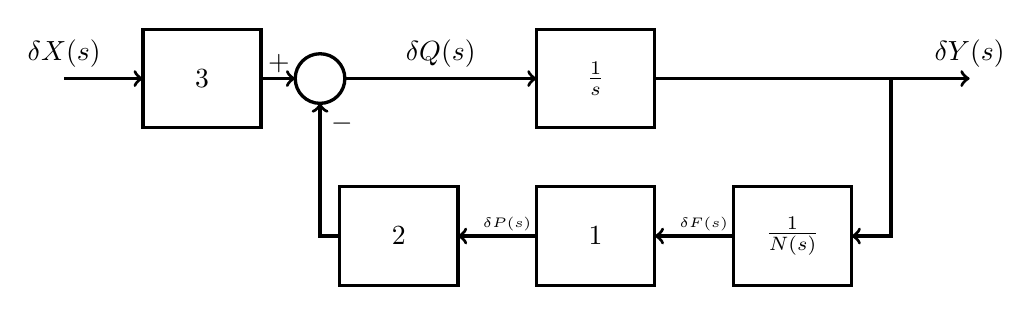
\begin{tikzpicture}[inner sep=0pt,outer sep=0pt,very thick,
sysblock/.style={draw,rectangle,inner sep=2pt,minimum width=1.5cm,minimum height=1.25cm,very thick}]

\draw (-1.5,0) node[sysblock] (d) {$3$};
\draw (0,0) node[draw,circle] (sum) {$\rule{0pt}{18pt}$};
\draw (3.5,0) node[sysblock] (a) {$\frac{1}{s}$};
\draw (3.5,-2) node[sysblock] (b) {$1$};
\draw (6,-2) node[sysblock] (b1) {$\frac{1}{N(s)}$};
\draw (1,-2) node[sysblock] (c) {$2$};

\draw[<-] (d.180)  -- ++(-1,0) node[above=4pt] {$\delta X(s)$};
\draw[->] (d.0) -- (sum.180) node[above left=2pt] {$+$};
\draw[->] (sum.0) -- node[pos=.5,above=4pt] {$\delta Q(s)$} (a.180);
\draw[->] (a.0) -- ++(4,0) node[above=4pt] {$\delta Y(s)$};
\draw[->] (a.0) -- ++(3,0) |- (b1.0);
\draw[->] (b1.180) node[above left=2pt] {\tiny$\delta F(s)$} -- (b.0);
\draw[->] (b.180) node[above left=2pt] {\tiny$\delta P(s)$} -- (c.0);
\draw[->] (c.180)  -| (sum.-90) node[below right=4pt] {$-$};

\end{tikzpicture}}
\end{center}


